The analysis is carried out for four configurations: full and narrow parameter ranges, each evaluated under \ac{nse} and logNSE. The results are organized by configuration below, with a comparative discussion at the end.

\vspace{0.5cm}
\noindent\textbf{Full parameter range with NSE}

Figure~\ref{fig:sobol_full_nse} shows the Sobol indices for all 17 parameters across the full admissible bounds. The total output variance is $V(Y) = 0.463$, which provides an adequately strong signal for reliable index estimation.

\begin{figure}[!ht]
\centering
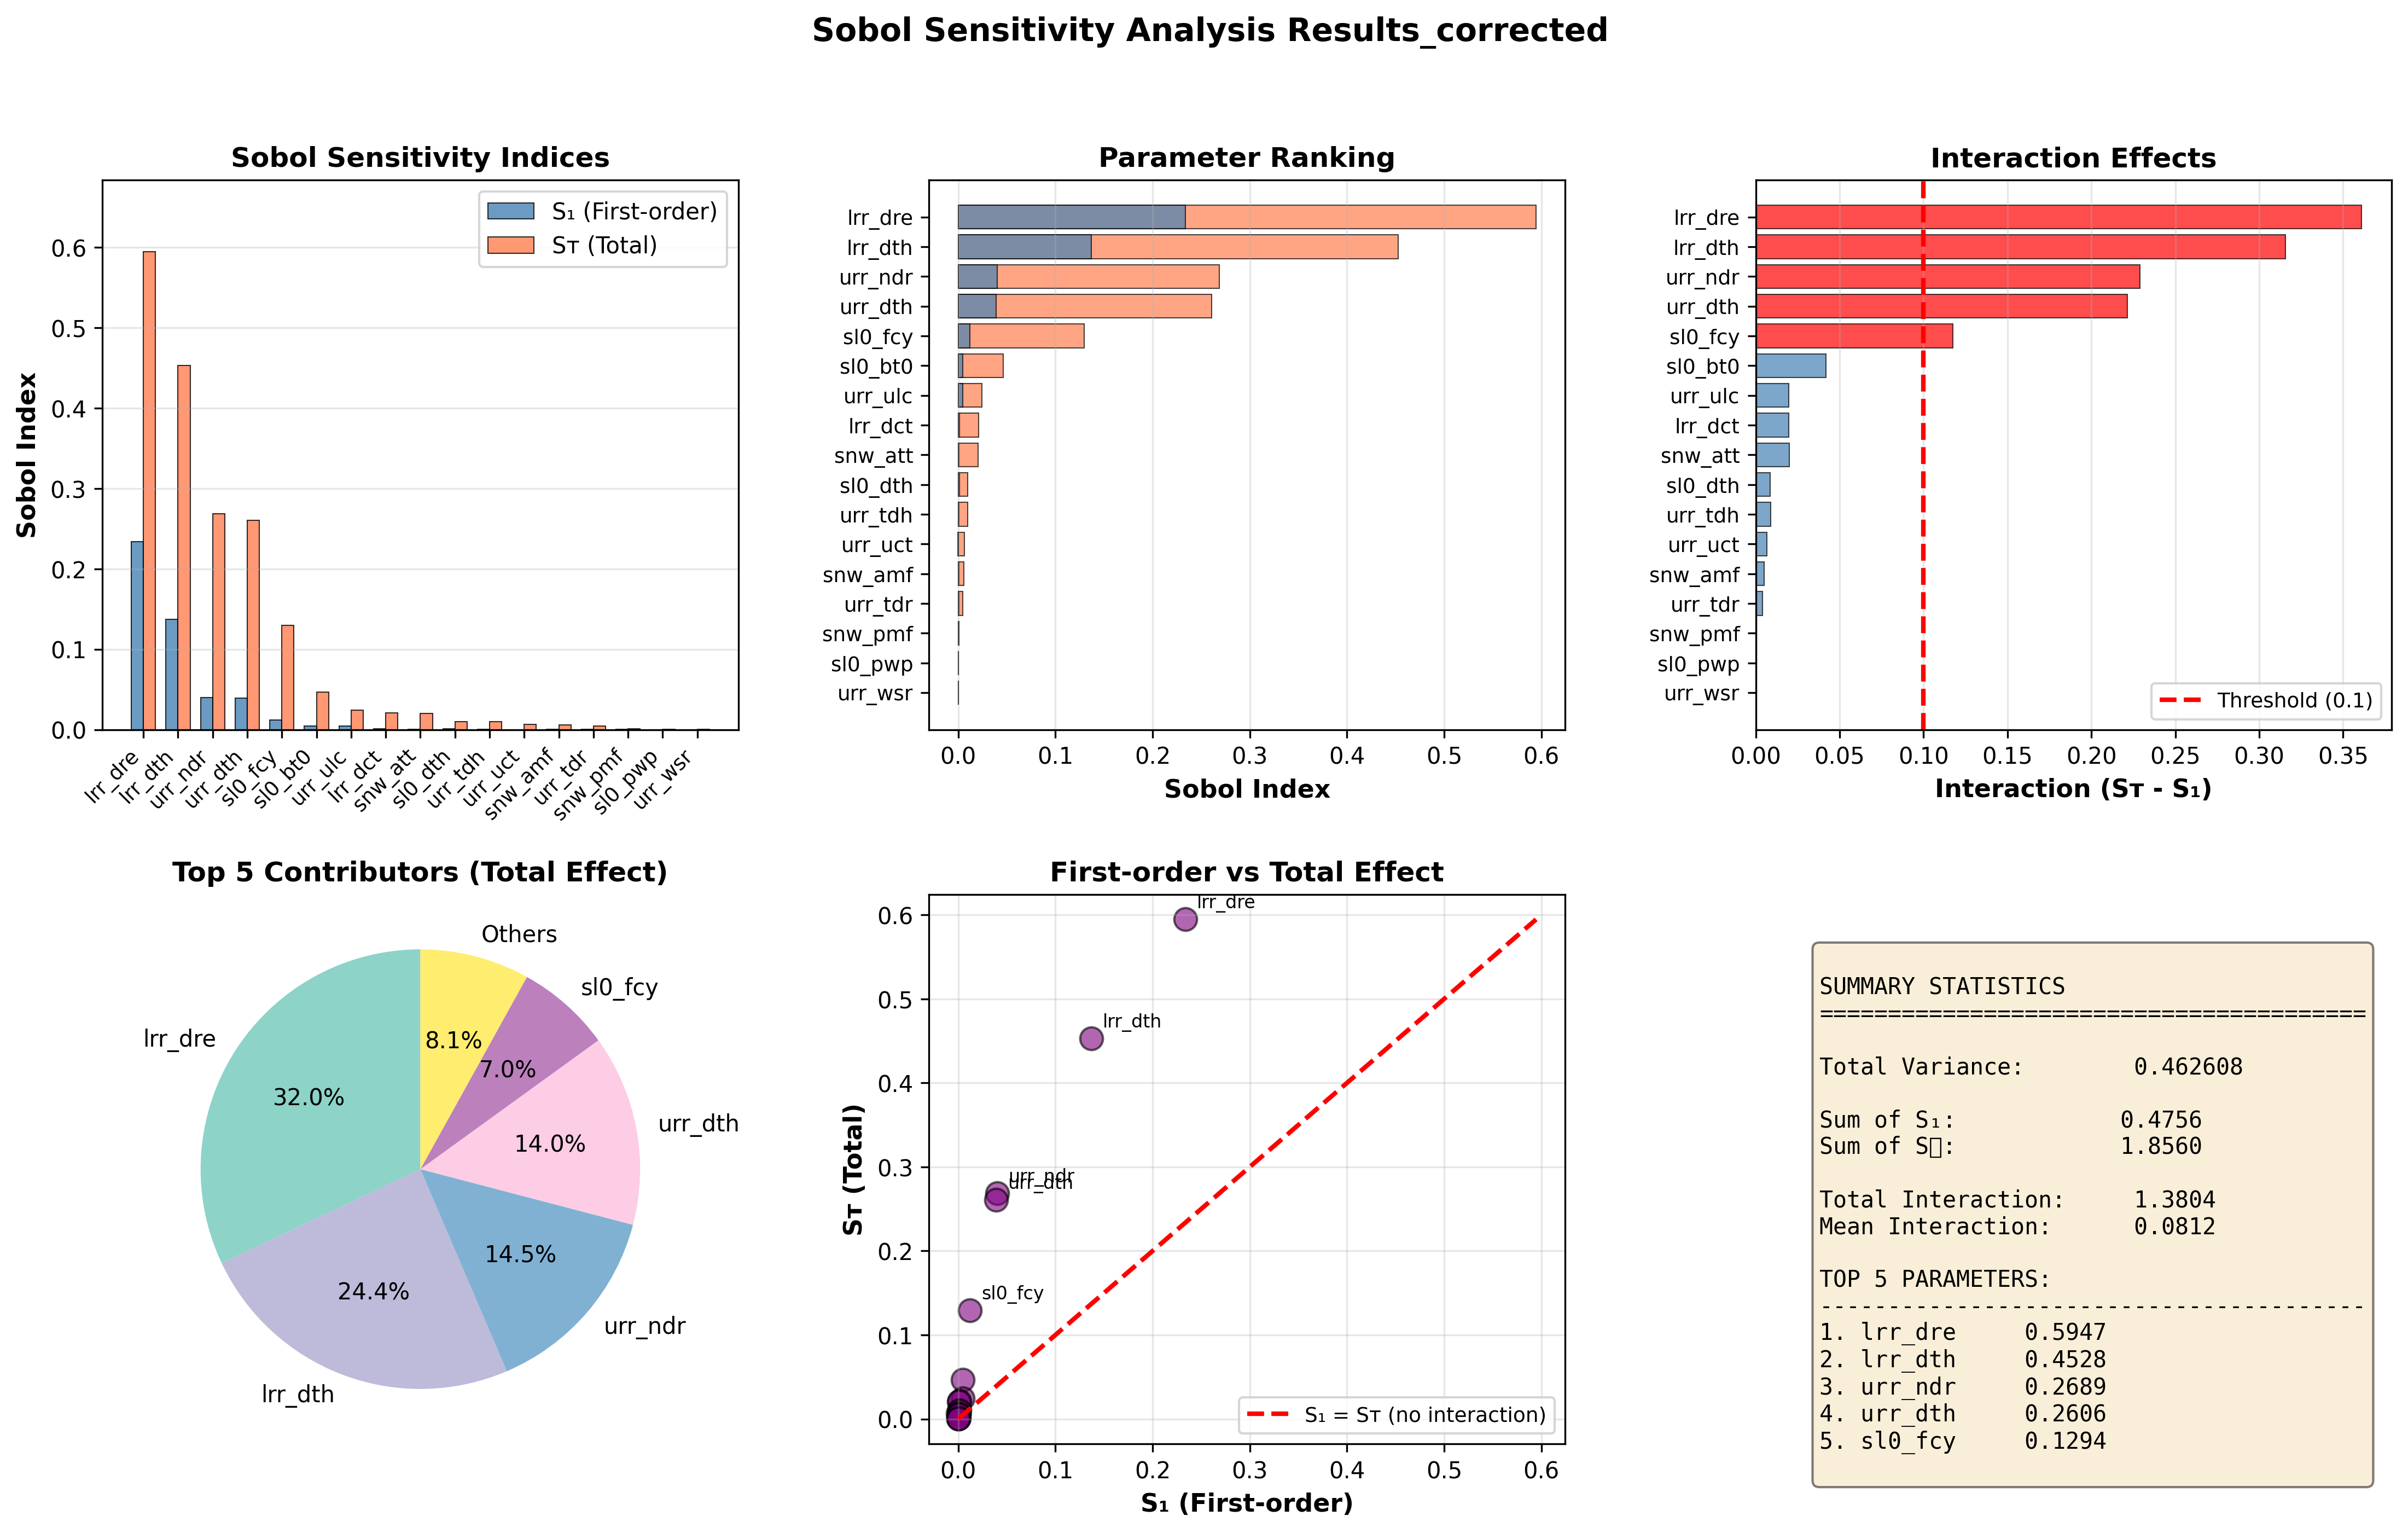
\includegraphics[width=0.90\textwidth]{Figures/Ass_03/sobol_full_range_nse.png}
\caption{First-order ($S_1$) and total-order ($S_T$) Sobol indices for all 17 \acp{mp} under \ac{nse} objective function and full parameter bounds. Parameters are sorted by $S_T$.}
\label{fig:sobol_full_nse}
\end{figure}

The lower reservoir parameters \texttt{lrr\_dre} ($S_T = 0.595$) and \texttt{lrr\_dth} ($S_T = 0.453$) are by far the most globally influential, followed by \texttt{urr\_ndr} ($S_T = 0.269$), \texttt{urr\_dth} ($S_T = 0.261$), and \texttt{sl0\_fcy} ($S_T = 0.129$). The sum of $S_T = 1.856$ substantially exceeds the sum of $S_1 = 0.476$, indicating strong parameter interactions: parameters do not act independently but jointly shape the output variance across the full space. Snow-related parameters (\texttt{snw\_pmf}, \texttt{snw\_amf}) contribute near-zero variance ($S_T < 0.001$), consistent with the rainfall-dominated nature of the event.

\vspace{0.5cm}
\noindent\textbf{Narrow parameter range with NSE}

Figure~\ref{fig:sobol_narrow_nse} shows results for the narrowed parameter range around the calibrated values.

\begin{figure}[!ht]
\centering
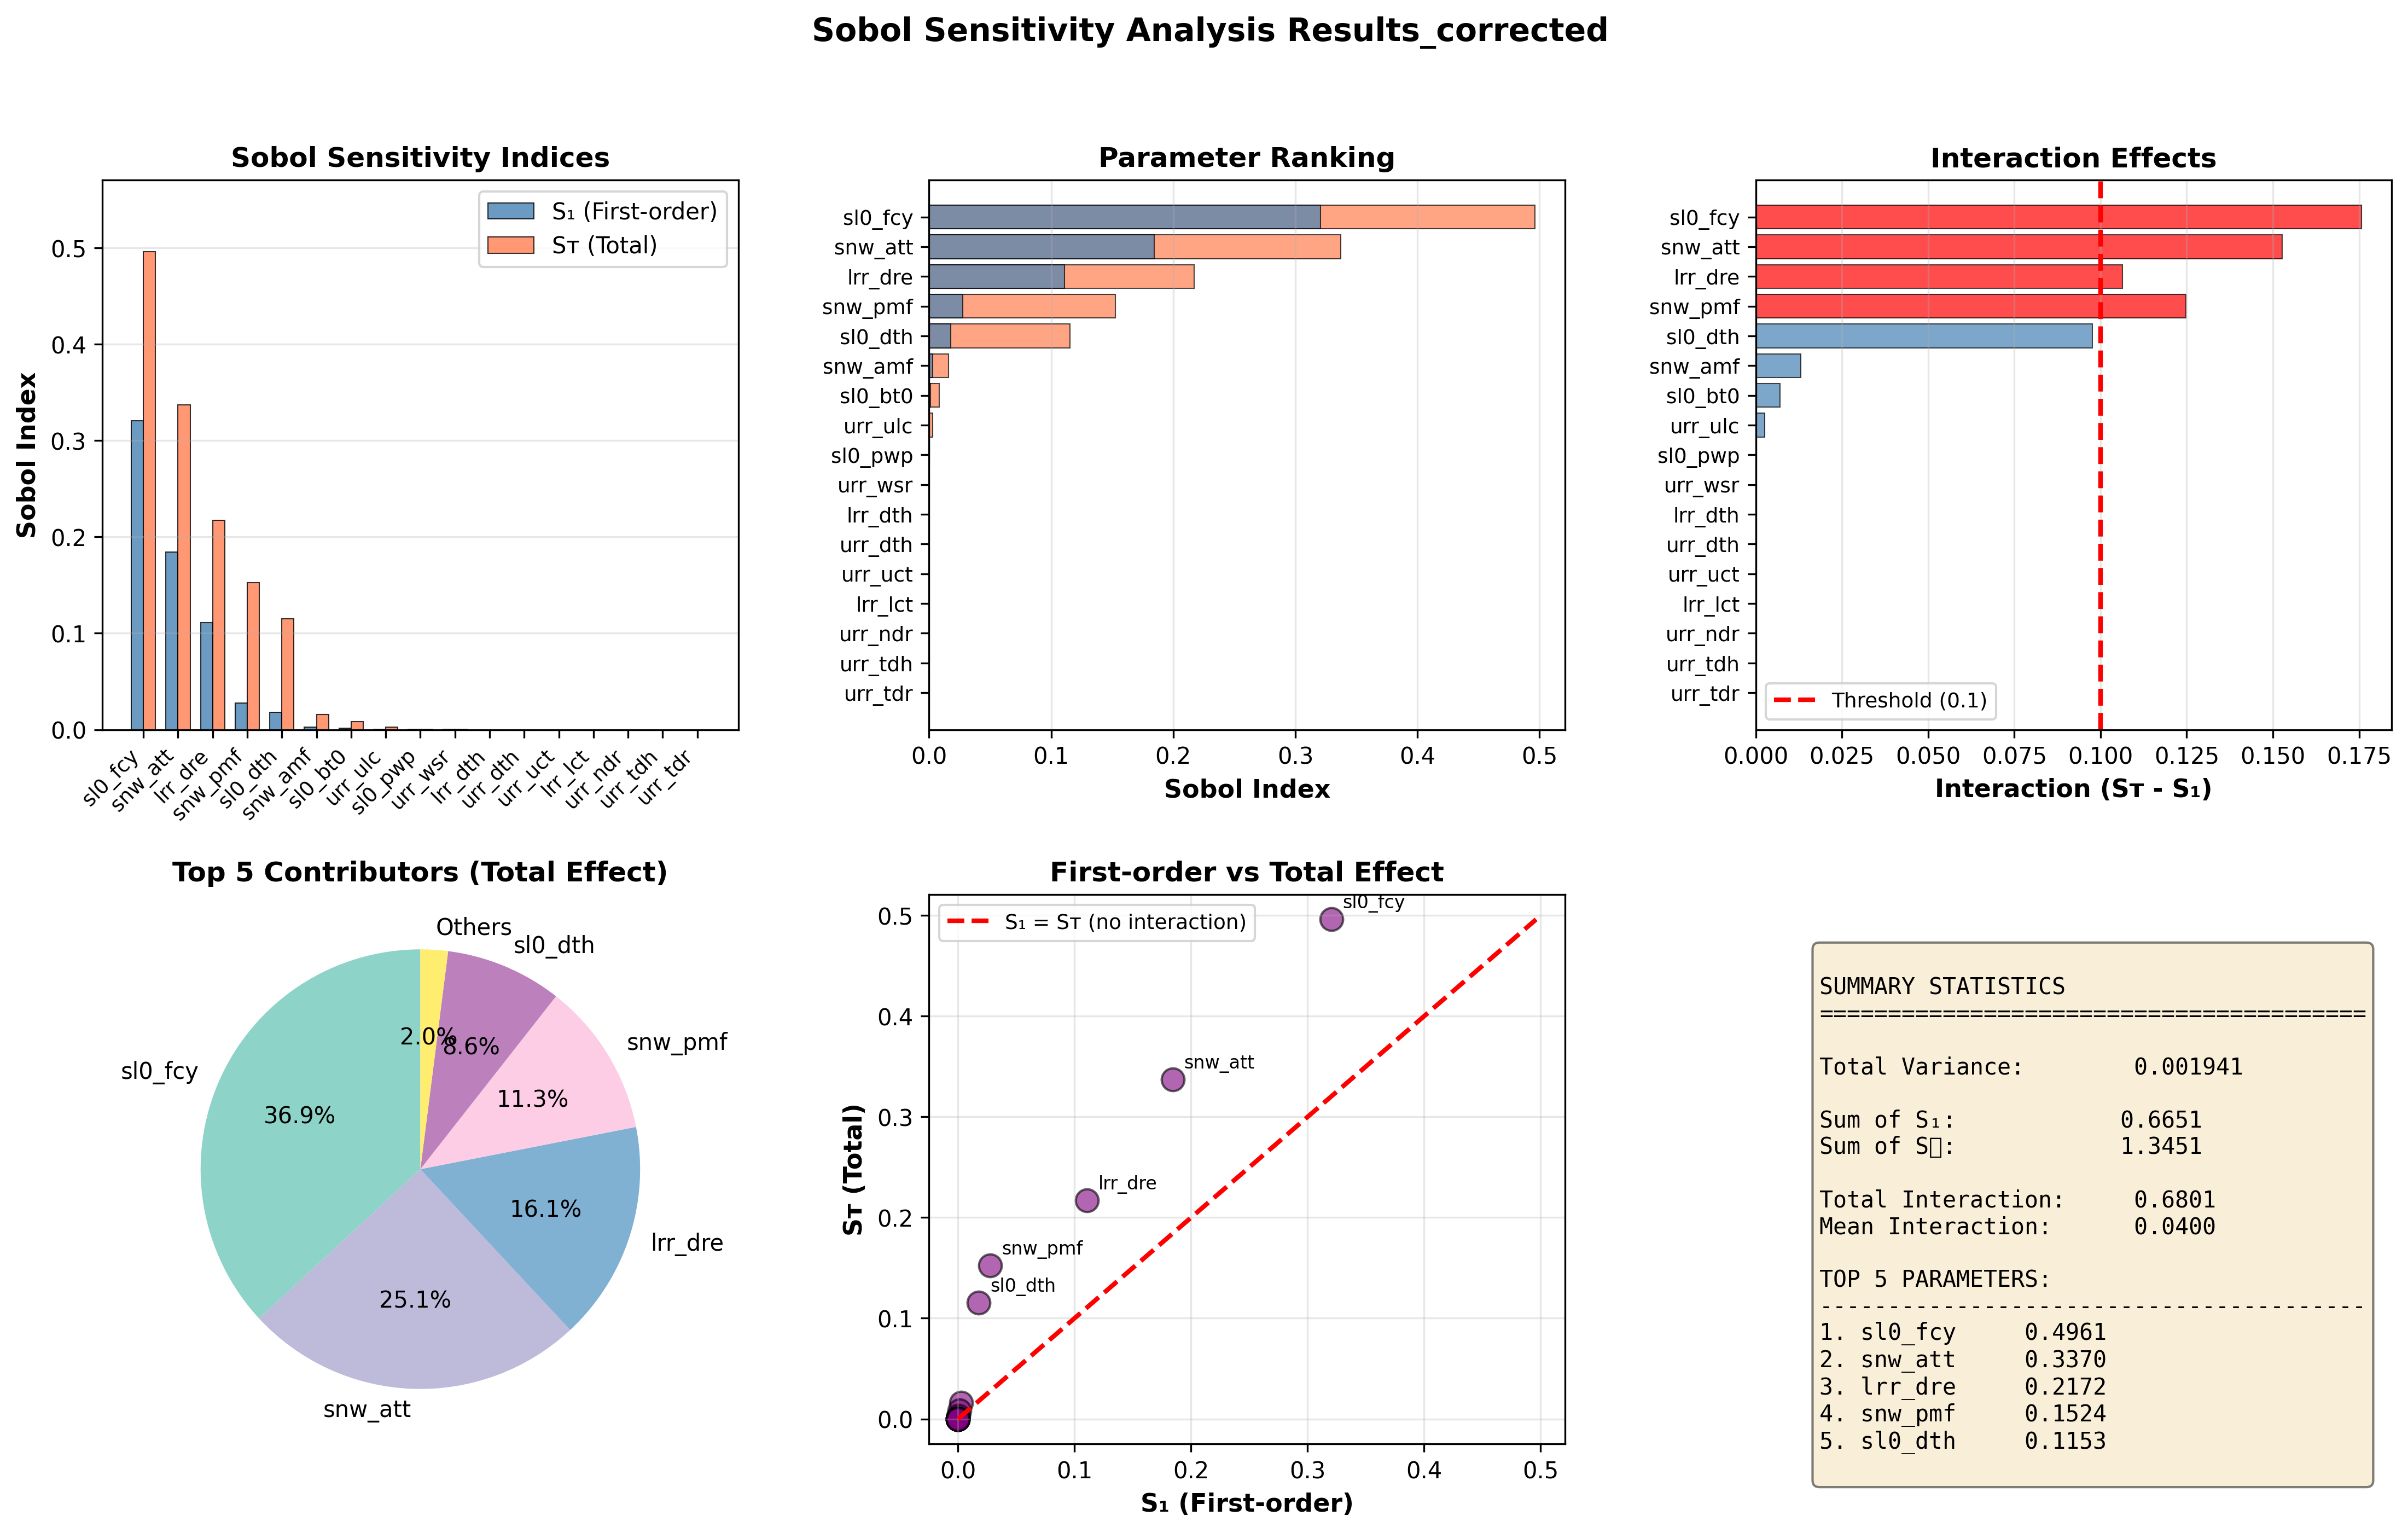
\includegraphics[width=0.90\textwidth]{Figures/Ass_03/new/sobol_analysis_corrected_narrow_NSE.png}
\caption{First-order ($S_1$) and total-order ($S_T$) Sobol indices under \ac{nse} and narrow parameter bounds.}
\label{fig:sobol_narrow_nse}
\end{figure}

The total variance drops sharply to $V(Y) = 0.0019$, reflecting that the model is well-behaved near the calibrated optimum and most parameter combinations in this region produce similar \ac{nse} values. With such a small total variance, the index estimates become susceptible to Monte Carlo noise. The leading parameters here are \texttt{sl0\_fcy} ($S_T = 0.496$), \texttt{snw\_att} ($S_T = 0.337$), and \texttt{lrr\_dre} ($S_T = 0.217$). Parameters \texttt{snw\_tdh} and \texttt{urr\_tdr} return $S_T = 0$, as their narrow bounds produce no detectable variation in the output. These results should be interpreted with caution, given the small denominator $V(Y)$.

\vspace{0.5cm}
\noindent\textbf{Narrow parameter range with logNSE}

Figure~\ref{fig:sobol_narrow_lognse} repeats the narrow-range analysis using logNSE.

\begin{figure}[!ht]
\centering
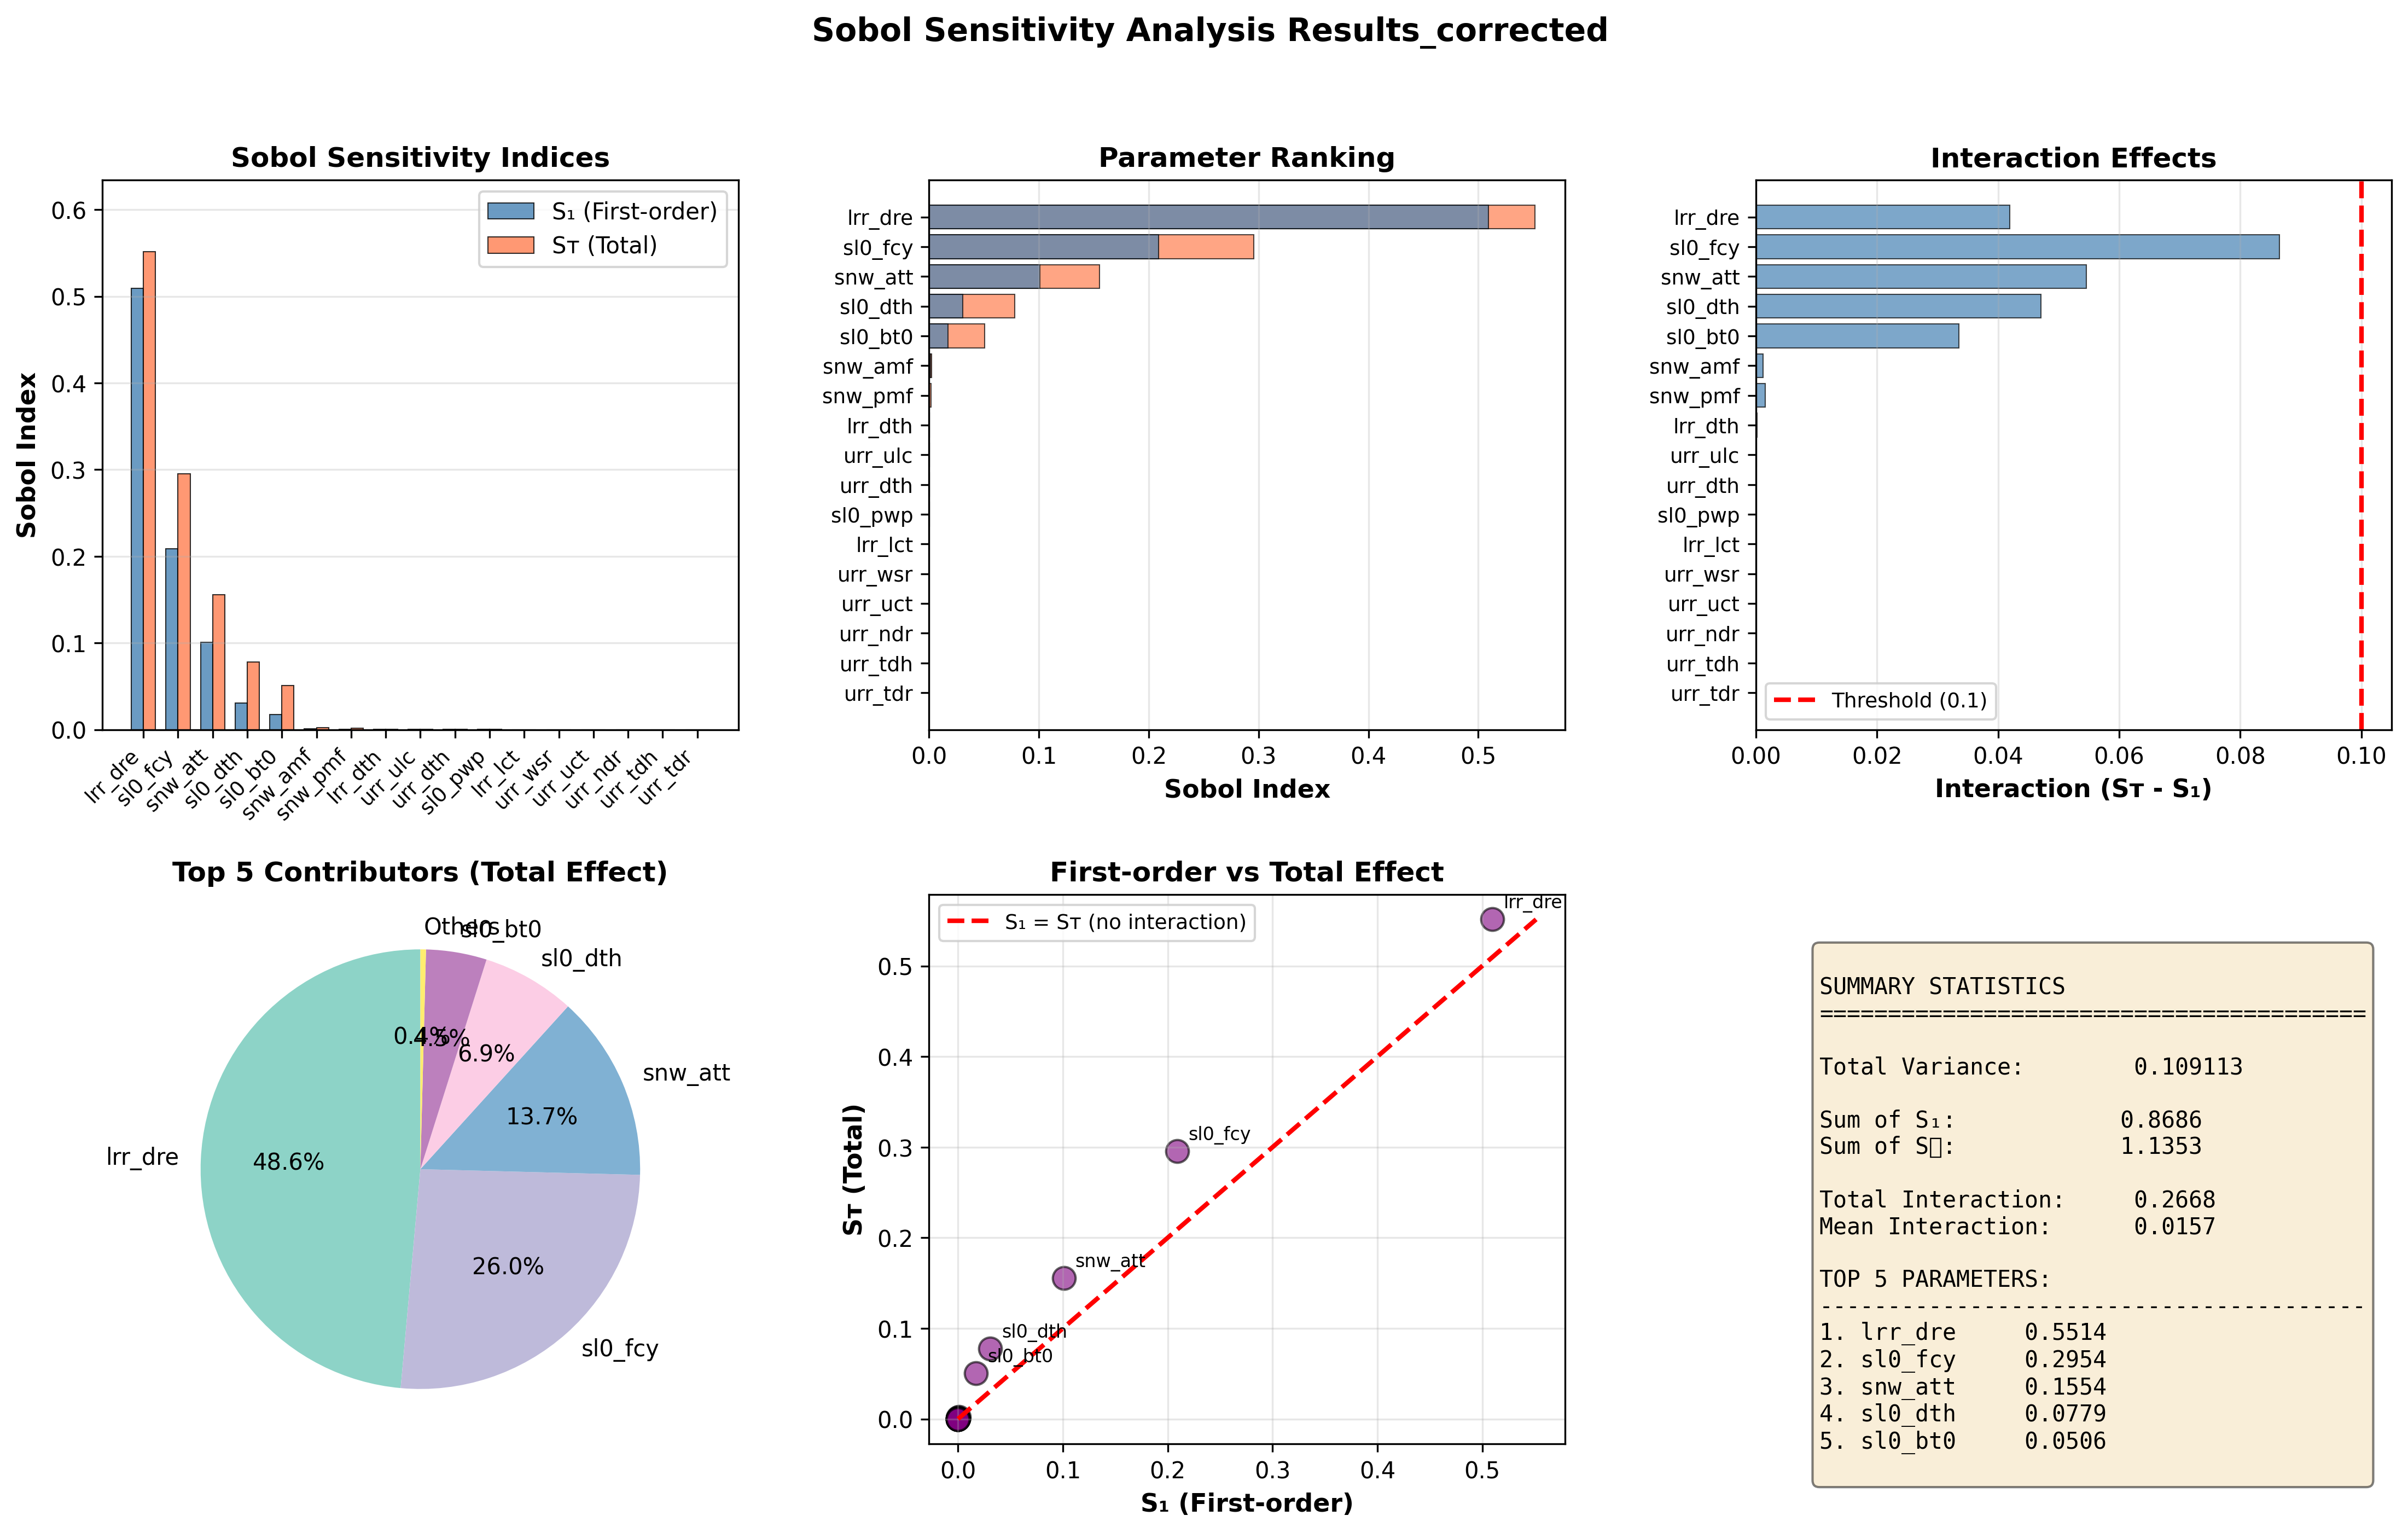
\includegraphics[width=0.90\textwidth]{Figures/Ass_03/new/sobol_analysis_corrected_narrow_logNSE.png}
\caption{First-order ($S_1$) and total-order ($S_T$) Sobol indices under logNSE and narrow parameter bounds.}
\label{fig:sobol_narrow_lognse}
\end{figure}

The total variance rises to $V(Y) = 0.109$ compared to $0.0019$ for NSE in the same range, because the log transformation amplifies relative differences in low-flow periods. The sum of $S_1 = 0.869$ and sum of $S_T = 1.135$ indicate small interaction effects; most variance is explained by first-order effects. \texttt{lrr\_dre} is overwhelmingly dominant ($S_1 = 0.510$, $S_T = 0.551$), confirming that the lower reservoir controls slow baseflow, which logNSE specifically targets. \texttt{sl0\_fcy}, \texttt{snw\_att}, \texttt{sl0\_dth}, and \texttt{sl0\_bt0} are the only other parameters with a meaningful contribution; all remaining parameters are essentially inactive under this metric and range.

\vspace{0.5cm}
\noindent\textbf{Full parameter range with logNSE (problematic run)}

Applying logNSE over the full parameter bounds produced numerically unreliable results, as shown in figure~\ref{fig:sobol_full_lognse_prob}. The total variance collapses to $V(Y) = 3.2 \times 10^{-5}$, and the sum of first-order indices reaches $\sum S_1 = 6.28$, which is physically impossible (valid Sobol indices by definition sum to at most 1 in the absence of interactions). The total-interaction term is also negative.

\begin{figure}[!ht]
\centering
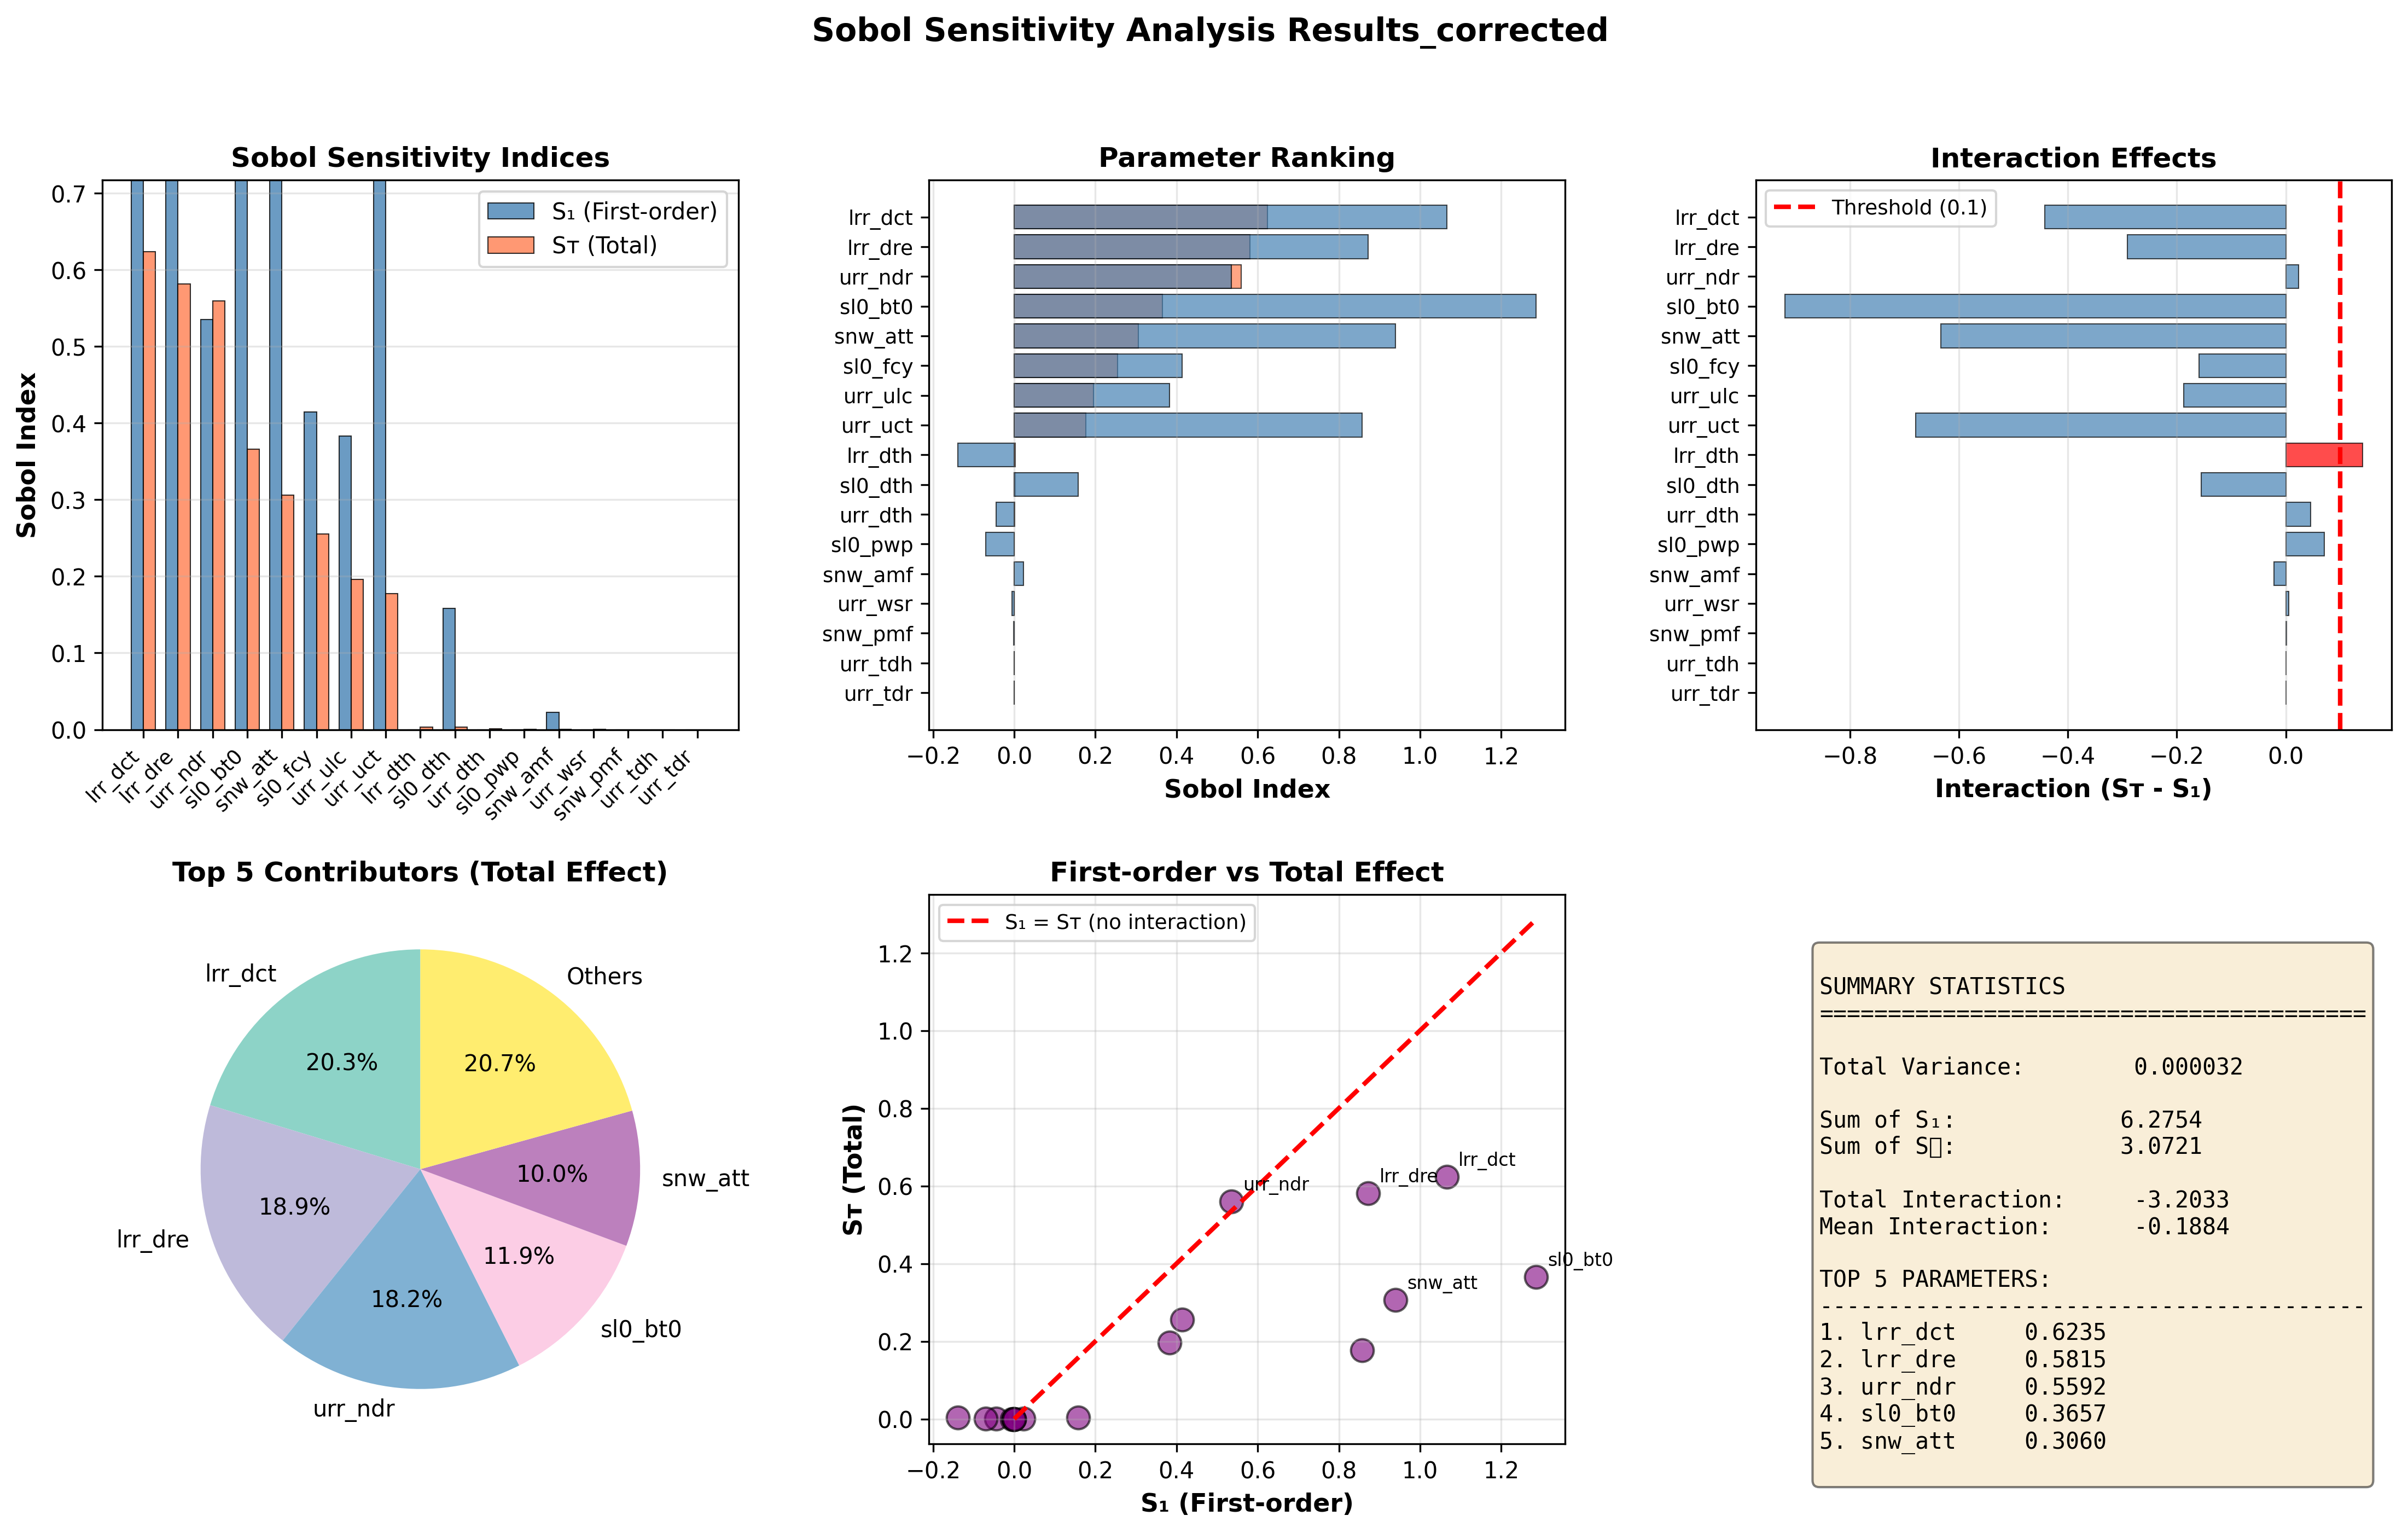
\includegraphics[width=0.90\textwidth]{Figures/Ass_03/sobol_full_range_lognse_problematic.png}
\caption{Sobol indices for the full parameter range under logNSE. This run is considered unreliable due to near-zero total variance and violation of $\sum S_1 \leq 1$.}
\label{fig:sobol_full_lognse_prob}
\end{figure}

The failure arises because many parameter combinations sampled from the full bounds produce model runs with near-zero simulated discharge at some time steps. The logarithm of near-zero values causes logNSE to diverge, effectively suppressing the output variance while simultaneously corrupting the variance decomposition. This result confirms that logNSE is not a suitable objective function for a full-range global \ac{sa} of this model; its use should be restricted to parameter ranges where all sampled runs produce physically plausible hydrographs.

\vspace{0.5cm}
\noindent\textbf{Comparison with local sensitivity analysis}

The full-range global \ac{sa} results reveal a slightly different picture from Assignment~2. In the local \ac{sa}, the soil parameters \texttt{sl0\_fcy} and \texttt{snw\_att}, and \texttt{lrr\_dre} were the dominant controls, while most upper reservoir parameters were completely insensitive. In the global \ac{sa}, \texttt{lrr\_dre} and \texttt{lrr\_dth} emerge as the most globally influential parameters. This contrast is not a contradiction: evaluated at the calibrated optimum, the lower reservoir is in a regime where its parameters produce negligible incremental change. But across the full parameter space, the lower reservoir structure determines how much water bypasses the fast surface pathway, controlling a large fraction of total output variance.

The findings also highlight that global \ac{sa} is strongly configuration-dependent. The choice of parameter range and objective function directly shapes which parameters appear sensitive. A narrow range near the calibrated point shrinks $V(Y)$ by a factor of roughly 440 compared to the full range under \ac{nse}, making results harder to interpret reliably. The logNSE objective provides useful additional insight only when applied over a parameter range that guarantees non-degenerate model outputs.
